\section{Algorithm}

\subsection{Phase Wrapping}
Four phase-shifted sinusoidal fringes were used in implementing PSP \cite{Chen2005}: 
\begin{align}
I_1(x,y)&=I_0(x,y) + I_{mod}(x,y)\cos{(\phi(x,y))}, \nonumber\\
I_2(x,y)&=I_0(x,y) + I_{mod}(x,y)\cos{(\phi(x,y)+\frac{\pi}{2})}, \nonumber\\
I_3(x,y)&=I_0(x,y) + I_{mod}(x,y)\cos{(\phi(x,y)+\pi)},\nonumber\\
I_4(x,y)&=I_0(x,y) + I_{mod}(x,y)\cos{(\phi(x,y)+\frac{3\pi}{2})},
\label{eq:four_fringes}
\end{align}  
where $I_0(x,y)$ is the average background intensity value, $I_{mod}(x,y)$ is the intensity value of the fringe pattern, and $I_i$, where $i=1,2,3,4$, is the intensity value of the $i^{th}$ image. To determine $I_0$ and $I_{mod}$, images of the fringe patterns projected to a reference plane and the actual object, respectively, are taken. 

To calculate the phase value $\phi(x,y)$, we express Eq.~(\ref{eq:four_fringes}) as 
\begin{align}
I_1(x,y)=I_0(x,y) + I_{mod}(x,y)\cos{(\phi(x,y))}, \nonumber\\
I_2(x,y)=I_0(x,y) - I_{mod}(x,y)\sin{(\phi(x,y))}, \nonumber\\
I_3(x,y)=I_0(x,y) - I_{mod}(x,y)\cos{(\phi(x,y))},\nonumber\\
I_4(x,y)=I_0(x,y) + I_{mod}(x,y)\sin{(\phi(x,y))}.
\label{eq:four_fringes2}
\end{align}  
Subtracting like terms, $I_2$ from $I_4$ and $I_3$ from $I_1$, we yield
\begin{align}
I_4(x,y)-I_2(x,y)&=2I_{mod}\sin{(\phi(x,y))}, \nonumber\\
I_1(x,y)-I_3(x,y)&=2I_{mod}\cos{(\phi(x,y))}.
\end{align}  
Dividing these two expressions, we get
\begin{equation}
\tan(\phi(x,y))=\frac{I_4-I_2}{I_1-I_3}.
\label{eq:tan_phase}
\end{equation}

Finally, the phase value is obtained by getting the inverse of Eq.~(\ref{eq:tan_phase}),
\begin{equation}
\phi(x,y)=\tan^{-1}{\left( \frac{I_4(x,y) - I_2(x,y)}{I_1(x,y)- I_3(x,y)}\right)}.
\label{eq:phase}
\end{equation}

Phase unwrapping is then performed to remove the discontinuities of the tangent inverse function at values near $2\pi$ by adding or subtracting multiples of $2\pi$.

\subsection{Phase Unwrapping}

Quality-guided path unwrapping algorithm by Herraez et al. was implemented for efficient phase unwrapping \cite{Herraez2002}. 
In Vergara's thesis in 2010, he used MATLAB's built-in \texttt{unwrap} function for the phase unwrapping part of PSP. He also made a Graphical User Interface (GUI) for the PSP which was consequently used by Sze \cite{Sze2012} in the 3D analysis of the Ticao stone in 2012.

The built-in \texttt{unwrap} function, however, was known to produce the singularities (as discussed in Section 1) as it unwraps in two directions (along the two dimensions). 
Its fixed data evaluation order is also unable to handle noisy images causing error to propagate faster.

The quality-guided path unwrapping algorithm, on the other hand, is determined by a pixel's reliability value based upon the gradients/differences of its neighboring pixels. Pixels with the highest reliability values are unwrapped first and the lowest-quality pixels last to prevent noise and error propagation \cite{Herraez2002}.
 
The second differences (D), which proves measurement for degree of concavity/convexity of a function is needed. Based on Figure \ref{fig:pixels}, D of an (i,j) pixel is computed as follows:

\begin{equation}
D(i,j) = {[H^2(i,j)+V^2(i,j) +{D_1}^2(i,j) + {D_2}^2(i,j)]}^{1/2}
\end{equation}
where
\begin{align}
H(i,j) &= \gamma[\phi(i-1,j)-\phi(i,j)]- \gamma[\phi(i,j)-\phi(i+1,j)] \\
V(i,j) &= \gamma[\phi(i,j-1)-\phi(i,j)]- \gamma[\phi(i,j)-\phi(i,j+1)] \\
D_1(i,j) &= \gamma[\phi(i-1,j-1)-\phi(i,j)]- \gamma[\phi(i,j)-\phi(i+1,j+1)] \\
D_2(i,j) &= \gamma[\phi(i-1,j+1)-\phi(i,j)]- \gamma[\phi(i,j)-\phi(i+1,j-1)]
\end{align}
and $\gamma$ is a simple unwrapping operation to remove any $2\pi$ steps between two consecutive pixels. D can be calculated for all pixels except for the borders which are processed last by setting their reliability value to infinity. The reliability of a pixel R is then defined as
\begin{equation}
R = 1/D.
\end{equation}

\captionsetup[figure]{width=5in}
\begin{figure}[h!]
	\centering
	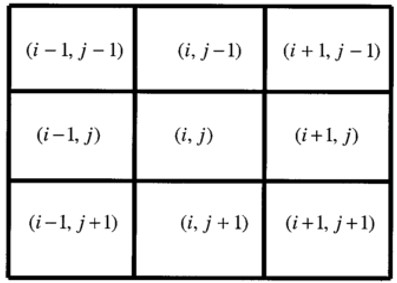
\includegraphics[width=0.4\textwidth]{figures/pixels.jpg}
	\caption[Calculation of second differences]{A 3x3 window illustration of the calculation of second difference of an (i,j) pixel \cite{Herraez2002}.}
	\label{fig:pixels}
\end{figure}

Unwrapping path is defined by the reliability of an edge which is  the summation of the reliabilities of the pixels that the edge connects (either vertical or horizontal) and not just the reliability of the pixel. The unwrapping path then proceeds to unwrap the pixels with the highest edge reliability value first \cite{Herraez2002}. 

A flowchart and complete explanation of this algorithm is found in Appendix A. This algorithm was already implemented in Python and is available in the \texttt{scikit-image} library. The code was just modified to fit our desired results.

The major difference, as well as the advantage, of this algorithm over the others is its \textit{discrete} or \textit{localized} unwrapping path, preventing noise to propagate throughout the image.

From the unwrapped phase maps, image processing techniques are further applied for enhancement of details which will be discussed in the following chapters.

\subsection{Phase To Height Conversion}

To determine the accuracy of the 3D reconstruction and the techniques applied, phase to height conversion is performed. We followed Wang and Du's algorithm \cite{Wang2009} for phase to height conversion.
%Thus, a 5-step pyramid excluding the reference plane was used throughout the calibration since it has discrete height values.

For the computation of the world height, given the image point $(x_i,y_i)$ and its corresponding phase value $\Phi$, the world height $z_w$ can be computed as 
\begin{equation}
	z_w=\frac{1+C_1 \Phi + ( C_2 + C_3 \Phi)x_i+ ( C_4 + C_5 \Phi)y_i}{D_0+D_1 \Phi + ( D_2 + D_3 \Phi)x_i + ( D_4 + D_5 \Phi)y_i},
	\label{eq:zw}
\end{equation}
where the coefficients $C_1$-$C_5$ and $D_0$-$D_5$ are the height calibration parameters to be determined. They are functions of the translational and rotational transformations of the camera and projection plane coordinates to world coordinates.

Physical determination of these coefficients is impractical and may lead to inaccurate results, thus the proposed method of determining the coefficients is through using a least-squares inverse approach. The least-squares error is expressed as 
\begin{equation}
	S=\sum\limits_{j=1}^m \left[\frac{1+C_1 \Phi_j + ( C_2 + C_3 \Phi_j)x_j + ( C_4 + C_5 \Phi_j)y_j}{D_0+D_1 \Phi_j + ( D_2 + D_3 \Phi_j)x_j + ( D_4 + D_5 \Phi_j)y_j} - z^g_j\right]^2,
	\label{eq:S}
\end{equation}
where $z^g_j$ denotes the absolute out-of-reference-plane heights of both the reference ($z = 0$) and calibration objects; $m$ is the total number of selected data points; larger $m$ yields higher accuracy. The coefficients in Eq.~(\ref{eq:S}) can be determined by using a  standard linear algorithm upon conversion of the nonlinear least-squares error to linear format. 

This least-squares problem can be recast to a matrix form by imposing Wiener's estimation. The parameters $C_1$-$C_5$ are computed first by selecting points on the reference plane, where $z^g_j$ are taken to be zero. In matrix form, it would look like
\begin{equation}
	\begin{pmatrix}
		-\Phi_j & -x_{i,j} & -x_{i,j}\Phi_j & -y_{i,j} & -y_{i,j}\Phi_j
	\end{pmatrix}
	\begin{pmatrix}
		C_1\\C_2\\C_3\\C_4\\C_5
	\end{pmatrix}
	=
	1.
	\label{eq:Ccoeff}
\end{equation}
or in shorthand notation, it can be written as
\begin{equation}
	\mathbf{UC}=\mathbf{1},
	\label{eq:Ccoeffshort}
\end{equation}
where $\mathbf{U}$ takes the form of the leftmost matrix in Eq.~(\ref{eq:Ccoeff}) but with $m$ number of rows, the right-hand side is an $m$ $x$ 1 column vector with all of its elements equal to one. Since there are five unknowns, at least five points ($m\geq5$) must be chosen to determine $\mathbf{C}$. Unknown $\mathbf{C}$ can then be solved by
\begin{equation}
	\mathbf{C}=(\mathbf{U^TU})^{-1}\mathbf{U^T1},
\end{equation}
where superscript $\mathbf T$ denotes transpose operation and superscript `-1' denotes an inverse matrix operation.

Once $C_1$-$C_5$ are determined, $D_0$-$D_5$ may now be computed through
\begin{align}
	\begin{pmatrix}
		z^g_k & z^g_k\Phi_k & z^g_k x_{i,k} & z^g_kx_{i,k}\Phi_k & z^g_k y_{i,k} & z^g_k y_{i,k}\Phi_k 
	\end{pmatrix}
	\begin{pmatrix}
		D_0\\D_1\\D_2\\D_3\\D_4\\D_5
	\end{pmatrix}
	\nonumber\\ \qquad \qquad= 
	\begin{pmatrix}
		1 + C_1\Phi_k + (C_2 + C_3\Phi_k)x_{i,k} + (C_4+C_5\Phi_k)y_{i,k}
	\end{pmatrix}
	.
	\label{eq:Dcoeff}
\end{align}
or in shorthand form, it may be expressed as
\begin{equation}
	\mathbf{WD}=\mathbf{V},
	\label{eq:Dcoeffshort}
\end{equation}
where $\mathbf{W}$ takes the form of the leftmost matrix in Eq.~(\ref{eq:Dcoeff}) but with $n\geq6$ rows and $\mathbf{V}$ is a column vector with $n$ elements.

Selecting $n\geq6$ points in the calibration objects and constructing the matrix $\mathbf W$ and vector $\mathbf V$, unknown $\mathbf{D}$ can be solved by
\begin{equation}
	\mathbf{D}=(\mathbf{W^TW})^{-1}\mathbf{W^TV}.
\end{equation}
At least two calibration objects of uniform but different heights or one calibration object with varying heights is needed to compute for $\mathbf{D}$.

Matrices C and D which contain all the coefficients needed are then plugged in to Eq.~(\ref{eq:zw}) to finally obtain the world height, $z_w$.